\section{Creació del dataset sintètic}
% Parlar de perquè necessitem un dataset sintètic
% Perque hem escullit aquest
% explicar el dataset, els seus camps, etc
% fer una anàlisi del dataset

Durant el desenvolupament i millora dels models del projecte, es va plantejar un repte important: la manca d'un conjunt complet de dades del món real. Les dades del món real són crucials per entrenar i avaluar models que puguin funcionar en aplicacions pràctiques. L'obtenció d'un \textit{dataset} prou ampli i divers per als models que es desenvolupen va ser un repte, ja que, com que no es disposava de les dades originals amb les quals s'hauria de treballar, es va haver de buscar un \textit{dataset} similar. La naturalesa sensible de les dades i restriccions de propietat associades als informes d'incidències dificulten la cerca d'un conjunt de dades similar.

Per tant, es va prendre la decisió d'utilitzar un \textit{dataset} sintètic, que és una col·lecció simulada de dades generades per imitar escenaris del món real. Tot i que no reprodueix les complexitats i matisos de les dades reals, les dades sintètiques serveixen com una valuosa eina per provar i refinar models quan les dades reals són inaccessibles o limitades.

\subsection{Descripció general}
El \textit{dataset} escollit és \textit{Named Entity Recognition in Indian court judgments} \cite{dataset} (Reconeixement d'Entitats Nomenades a Sentències Judicials de l'Índia). Aquest \textit{dataset} sintètic és una col·lecció seleccionada de sentències judicials que han sigut anotades centrant-se en entitats amb més rellevància dins del context judicial. Aquesta elecció ha estat guiada per les següents consideracions que l'han convertit en un candidat adequat per avaluar el rendiment dels models:

\begin{itemize}
  \item \textbf{Entitats complexes:} Les sentències dels tribunals indis solen contenir terminologia jurídica complexa, noms diversos i algunes entitats llargues que suposen un repte per als sistemes NER. Aquesta complexitat proporciona un terreny de proves per als models, cosa que permet avaluar la seva capacitat per extreure amb precisió entitats intricades i variades, tal com apareixen als tiquets reals.
  \item \textbf{Sensibilitat al context:} El conjunt de dades escollit fa especial èmfasi en la importància del context en el reconeixement d'entitats. En els documents jurídics, els noms es poden referir a múltiples entitats en funció del context, una característica que reflecteix els reptes s'esperava trobar al conjunt de tiquets proporcionats per l'\textbf{Agència}. Aquesta consideració s'alineava amb les complexitats contextuals que preveiem en escenaris d'incidències on una única entitat (per exemple, una adreça de correu electrònic) pot representar diferents papers (atacant, destinatari, usuaris afectats) en funció del context. Comprendre i abordar aquests matisos específics del context ha sigut crucial per al desenvolupament de models precisos.
\end{itemize}


\subsection{Visió general de les dades}
Per com funcionen els judicis a l'Índia, una sentència típica d'un tribunal es pot dividir en dues parts: el preàmbul i la sentència. La separació entre el preàmbul i la sentència sol estar marcat per una paraula clau com ``JUDGMENT'' o ``ORDER''. 
\begin{itemize}
  \item \textbf{Preàmbul:} El preàmbul d'una sentència conté les dades importants de la sentència tals com els noms de les parts, jutges, advocats, etc. Aquestes dades no solen tenir frases gramaticalment completes, sinó que estan formatades.
  \item \textbf{Sentència:} Per altra banda, el text que segueix el preàmbul fins al final de la sentència es diu simplement ``sentència''.
\end{itemize}
Per a l'ús que se li ha donat, s'ha considerat que els preàmbuls i les sentències poden ser combinades en el mateix conjunt de dades per aconseguir més dades i més diversitat.

El \textit{dataset} conté les següents entitats extretes:
\begin{itemize}
  \item \textbf{TRIBUNAL:} Nom de qualsevol tribunal esmentat.
  \item \textbf{SOL·LICITANT:} Nom dels sol·licitants del cas actual.
  \item \textbf{DEMANDAT:} Nom dels demandats/acusats/oposició del cas actual.
  \item \textbf{JUTGE:} Nom dels jutges del cas actual i dels casos anteriors.
  \item \textbf{ADVOCAT:} Nom dels advocats d'ambdues parts.
  \item \textbf{DATA:} Qualsevol data esmentada a la sentència.
  \item \textbf{ORG:} Nom de les organitzacions esmentades al text a part del tribunal.
  \item \textbf{GPE:} Llocs geopolítics que inclouen noms d'estats, ciutats i pobles.
  \item \textbf{ESTATUT:} Nom de la llei esmentada a la sentència.
  \item \textbf{DISPOSICIÓ:} Seccions, subseccions, articles, lleis, normes d'un estatut.
  \item \textbf{PRECEDENT:} Tots els casos judicials anteriors referits a la sentència com a precedent.
  \item \textbf{NÚMERO\_CAS:} Tots els altres números de casos esmentats a la sentència (a part del precedent).
  \item \textbf{TESTIMONI:} Nom dels testimonis de la sentència actual.
  \item \textbf{ALTRES\_PERSONES:} Nom de totes les persones no catalogades com a \linebreak sol·licitant, demandat, jutge, advocat o testimoni.
\end{itemize}



\subsection{Preprocessament del dataset}
El \textit{dataset} originalment està en format \texttt{.json}, un format que pot ser còmode per la tasca de NER, però per generació de text és més útil tenir-ho en altres formats. Per transformar el conjunt de dades en format \texttt{.csv} s'han executat els següents passos:

\begin{enumerate}
  \item \textbf{Llegir el \textit{dataset}:} Per començar, s'ha carregat el \textit{dataset} des dels fitxers JSON on s'emmagatzemen les dades utilitzant la llibreria \texttt{json}.
  \item \textbf{Unir totes les sentències:} Les sentències i els preàmbuls que estaven en arxius diferents s'han unit en la mateixa variable, pel motiu mencionat anteriorment.
  \item \textbf{Escriure la capçalera:} La capçalera d'un arxiu \texttt{.csv} és el títol de les columnes. En aquest cas ha sigut ``sentence'' i ``output'' pel text d'entrada i les entitats de sortida, respectivament.
  \item \textbf{Iterar per les sentències:} Cada sentència conté un camp identificador, un d'anotacions, un de dades i un de metadades.
  \item \textbf{Escriure el text:} S'ha escrit el text en el fitxer de sortida amb el format esperat per un \texttt{.csv}.
  \item \textbf{Recórrer les anotacions:} S'ha iterat per cada anotació d'una sentència on hi ha les entitats extretes del text.
  \item \textbf{Escriure les entitats:} Cada entitat, ha sigut escrita a la seva categoria separada per comes. En cas que un tipus d'entitat no tingui cap entrada, s'ha escrit \pyth{'#not_found#'}.
\end{enumerate}

Aquest procés s'ha repetit pels arxius de \textit{train} i de \textit{test}, que estaven separats. Addicionalment, s'ha separat 1000 entrades de l'arxiu \textit{train} en un anomenat \textit{validation} per tenir tots els arxius necessaris per a l'entrenament.



\subsection{Exploració de les dades}

\subsubsection{Recompte d'entitats per tipus}
A partir del nombre d'entitats recopilades mostrades a la taula \ref{tab:recompte_entitats}, es va veure que cap entitat domina el conjunt de dades, i que la distribució està relativament equilibrada entre les diferents classes. Encara que hi ha algunes variacions, cap dels tipus d'entitat té una majoria ni està gaire infrarepresentat.

\begin{table}[H]
    \centering
    \begin{tabular}{lccr}
        \Xhline{2\arrayrulewidth}
        Entitat & Recompte Sentències & Recompte Preàmbuls & Total \\
        \hline
        \textbf{TRIBUNAL} & 1293 & 1074 & \textbf{2367} \\
        \textbf{SOL·LICITANT} & 464 & 2604 & \textbf{3068} \\
        \textbf{DEMANDAT} & 324 & 3538 & \textbf{3862} \\
        \textbf{JUTGE} & 567 & 1758 & \textbf{2325} \\
        \textbf{ADVOCAT} & NA & 3505 & \textbf{3505} \\
        \textbf{DATA} & 1885 & NA & \textbf{1885} \\
        \textbf{ORG} & 1441 & NA & \textbf{1441} \\
        \textbf{GPE} & 1398 & NA & \textbf{1398} \\
        \textbf{ESTATUT} & 1804 & NA & \textbf{1804} \\
        \textbf{DISPOSICIÓ} & 2384 & NA & \textbf{2384} \\
        \textbf{PRECEDENT} & 1351 & NA & \textbf{1351} \\
        \textbf{NÚMERO\_CAS} & 1040 & NA & \textbf{1040} \\
        \textbf{TESTIMONI} & 881 & NA & \textbf{881} \\
        \textbf{ALTRES\_PERSONES} & 2653 & NA & \textbf{2653} \\
        \hline
        \textbf{Total} & 17485 & 12479 & \textbf{29964} \\
        \Xhline{2\arrayrulewidth}
    \end{tabular}
    \caption[Recompte de les entitats en les sentències, els preàmbuls i en total.]{Recompte de les entitats recopilades en les sentències, els preàmbuls i en total.}
    \label{tab:recompte_entitats}
\end{table}

L'equilibri entre les classes d'entitats es pot veure més clarament en la figura \ref{fig:diagrama_sectors_tipus_entitats} on es compara percentualment la proporció d'entitats al \textit{dataset}.
\begin{figure}[H]
  \centering
  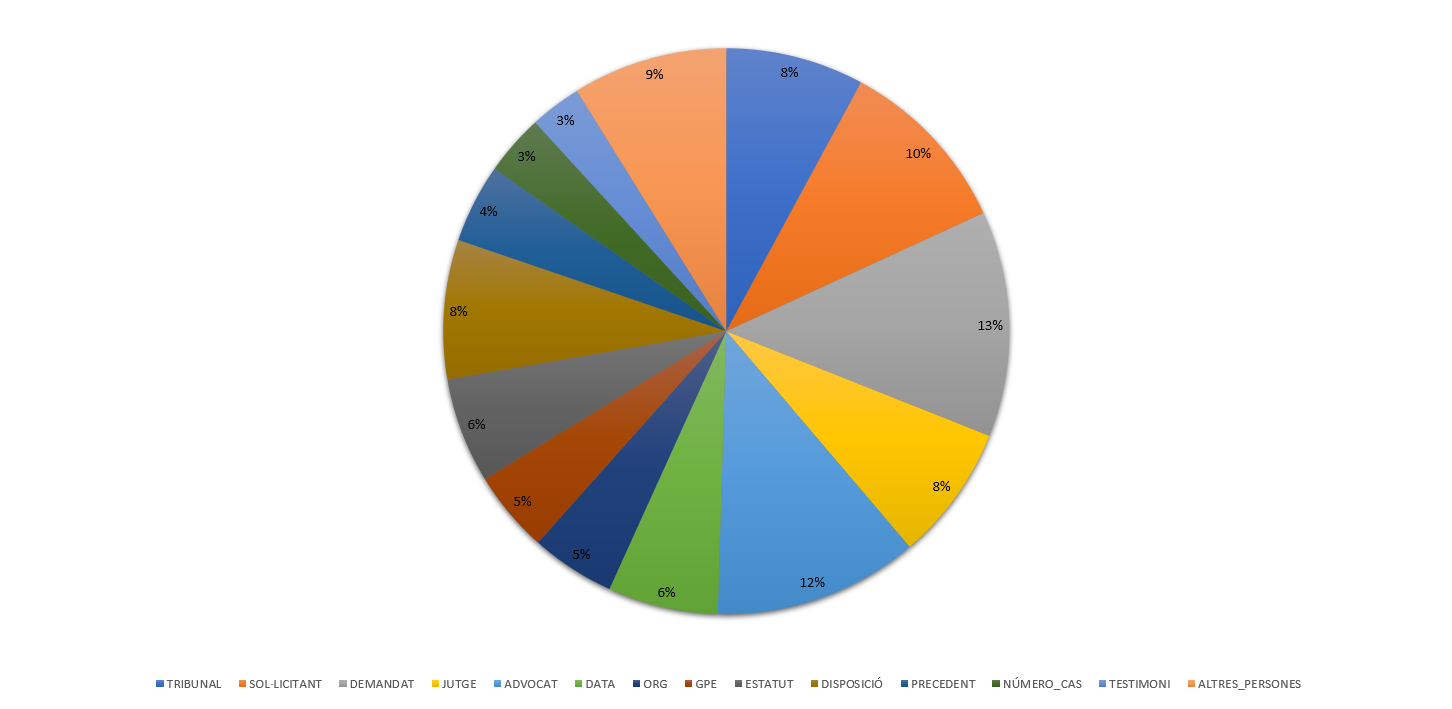
\includegraphics[width=\textwidth]{formatge_tipus_entitats.png}
  \caption[Diagrama de sectors del nombre d'entitats a les sentències]{Diagrama de sectors comparant el nombre d'entitats a les sentències. \\ (Creació pròpia)}
  \label{fig:diagrama_sectors_tipus_entitats}
\end{figure}

\subsubsection{Recompte de sentències per tipus de cas i per tribunal}
A l'hora de recopilar les sentències, és probable que les sentències més esmentades siguin les més importants. Però limitar-se a prendre les sentències més citades d'un determinat tribunal donaria lloc a un biaix en determinats tipus de casos (per exemple, casos criminals). Per tant, cal controlar els tipus de casos per tenir en compte la varietat de sentències. Així doncs, al \textit{dataset} hi ha els 8 tipus de casos més freqüents: civils, constitucionals, criminals, financers, industrials i laborals, de terreny i propietat, de vehicles i d'impostos.

Per mostrar que aquesta distribució és equilibrada, es pot veure el recompte fet a la taula \ref{tab:distribucio_cas_tribunal}, on es mostra el recompte de les sentències per tipus de cas i per tribunal de les sentències.


\subsubsection{Recompte de sentències per llargada}
A l'exploració del conjunt de dades, un aspecte que ha cobrat importància és la distribució de les longituds de les sentències. Aquesta anàlisi proporciona informació sobre la variabilitat de les longituds d'entrada i ha ajudat a descobrir l'estructura general i els possibles \textit{outliers} o valors atípics del conjunt de dades.

En primer lloc, es va generar un \textit{boxplot} (diagrama de caixa) per visualitzar les longituds dels texts d'entrada del \textit{dataset} com es pot veure a la figura \ref{fig:box_longitud_sentencies_tot}. El diagrama de caixa va revelar un valor atípic: una sentència que era significativament més llarga que totes les altres. Es va descobrir que aquesta frase era un error, i que no tenia sentit. A més a més, es van identificar quatre sentències atípiques les quals superaven els 4.000 caràcters. Es va decidir eliminar aquests valors atípics per evitar anàlisis esbiaixades i garantir que el model s'entreni amb dades representatives i significatives.

\begin{figure}[H]
  \centering
  \begin{subfigure}{.5\textwidth}
    \centering
    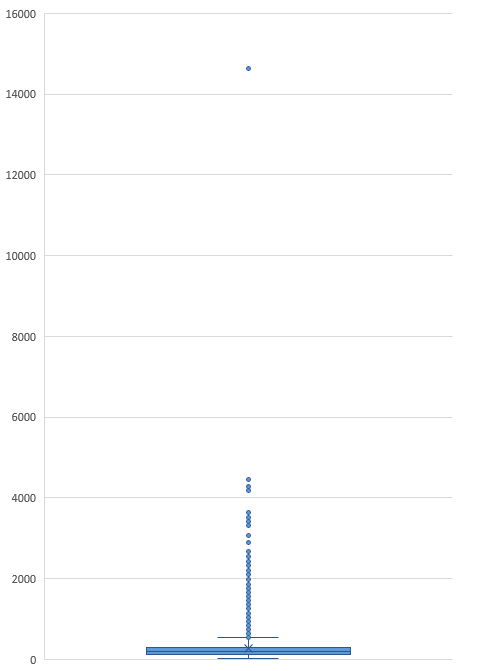
\includegraphics[width=.7\linewidth]{box_sent.png}
    \caption{Amb totes les sentències.}
    \label{fig:box_longitud_sentencies_tot}
  \end{subfigure}%
  \begin{subfigure}{.5\textwidth}
    \centering
    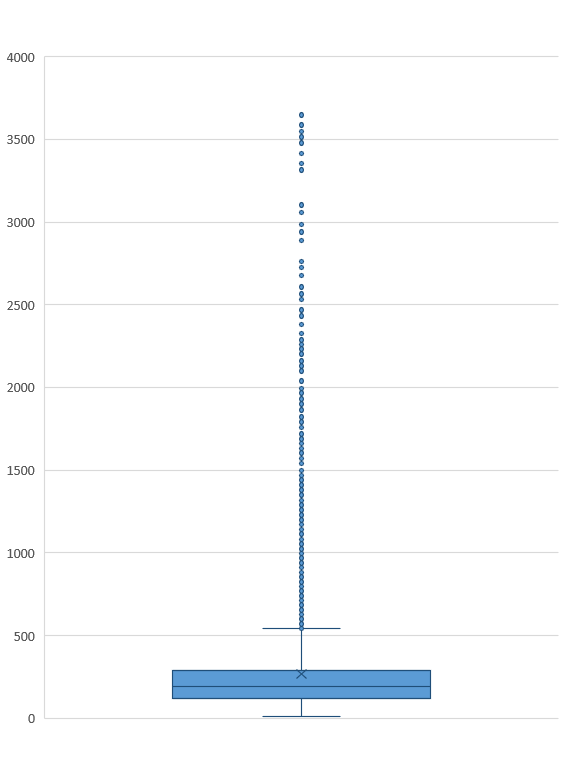
\includegraphics[width=.7\linewidth]{box_sent_out.png}
    \caption{Sense \textit{outliers}.}
    \label{fig:box_longitud_sentencies_out}
  \end{subfigure}
  \caption[Boxplot de la longitud de les sentències]{Boxplot de la longitud de les sentències, abans i després d'eliminar els \textit{outliers}. \\ (Creació pròpia)}
  \label{fig:box_longitud_sentencies}
\end{figure}

Després d'eliminar els valors atípics identificats, es va generar un nou \textit{boxplot} per visualitzar la nova distribució de la longitud de les frases \ref{fig:box_longitud_sentencies_out}. 

Addicionalment, a la figura \ref{fig:histograma_sentencies_out} es pot veure que s'ha creat un histograma per oferir una visió més detallada de la distribució de freqüències dins dels diferents rangs de longitud.

\begin{figure}[H]
  \centering
  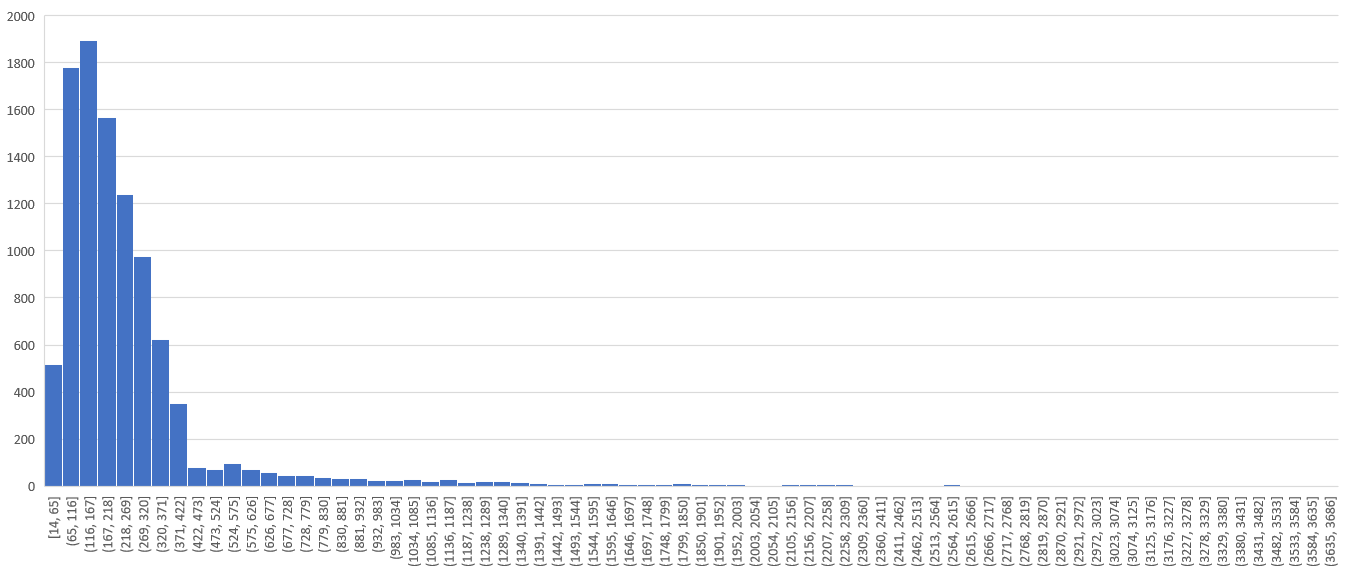
\includegraphics[width=\textwidth]{hist_sent_out.png}
  \caption[Histograma de la longitud de les sentències]{Histograma de la longitud de les sentències, sense \textit{outliers}. \\ (Creació pròpia)}
  \label{fig:histograma_sentencies_out}
\end{figure}


\subsubsection{Recompte d'entitats per llargada}
L'anàlisi de la longitud de les entitats proporciona informació sobre l'estructura i la composició del \textit{dataset}, revelant possibles patrons i anomalies. L'histograma a la figura \ref{fig:histograma_entitats_tipus} il·lustra la distribució de les longituds de les entitats entre els diferents tipus. Cada barra representa un interval de longituds de dos caràcters per un tipus concret d'entitat, i l'alçada de la barra indica el recompte d'entitats compreses en aquest interval de longitud.

Observant la figura \ref{fig:histograma_entitats_tipus} es pot veure que la categoria ``DEMANDAT'' ha destacat per mostrar un nombre significatiu d'entitats amb longituds superiors o iguals a 100 caràcters.

\begin{figure}[H]
  \centering
  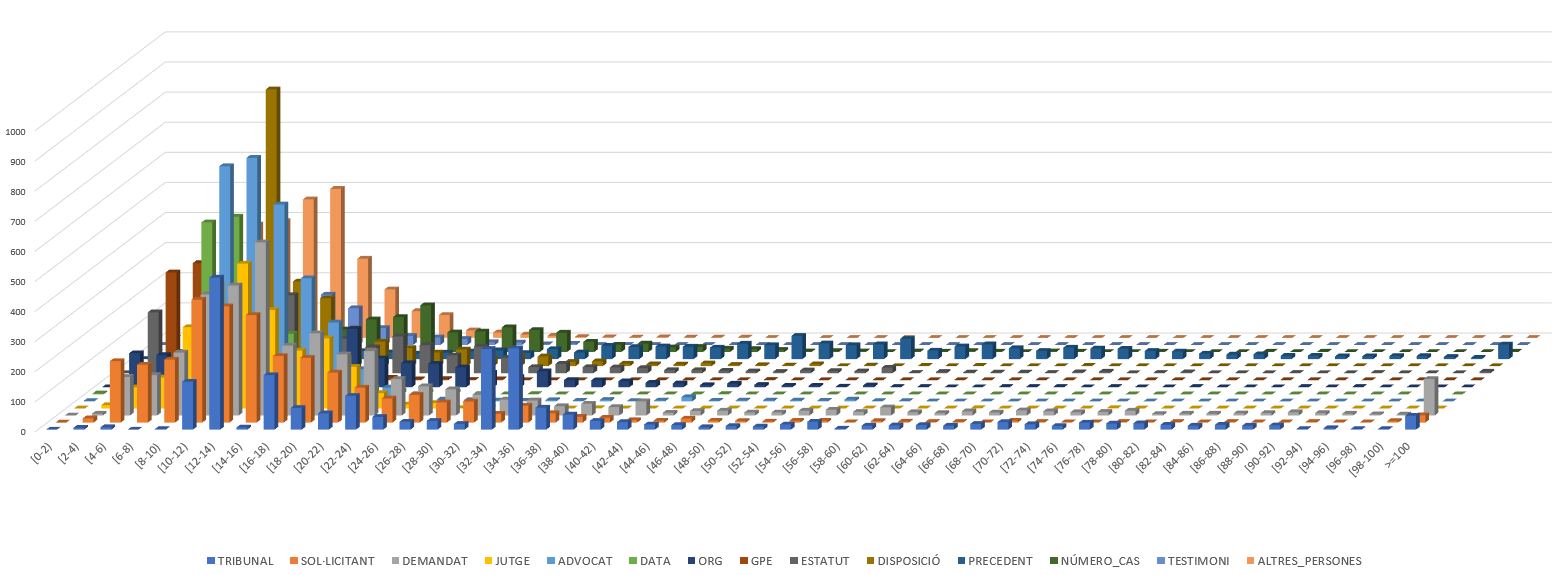
\includegraphics[width=\textwidth]{hist_ent_categoria.png}
  \caption[Histograma de la longitud de les entitats, per categoria]{Histograma de la longitud de les entitats, per categoria. \\ (Creació pròpia)}
  \label{fig:histograma_entitats_tipus}
\end{figure}

Tal com es veu la figura \ref{fig:histograma_entitats_total}, s'ha generat també un histograma complet combinant tots els tipus d'entitats. L'histograma unificat proporciona una visió global de la distribució de la longitud a tot el \textit{dataset}. Les entitats de diferents categories tendeixen a tenir una longitud semblant. Més concretament, el 55\% de les entitats tenen entre 8 i 18 caràcters i el 90\% de les entitats en tenen menys de 36. Aquesta uniformitat en la distribució de la longitud suggereix que les entitats es representen de forma coherent en el \textit{dataset}.

\begin{figure}[H]
  \centering
  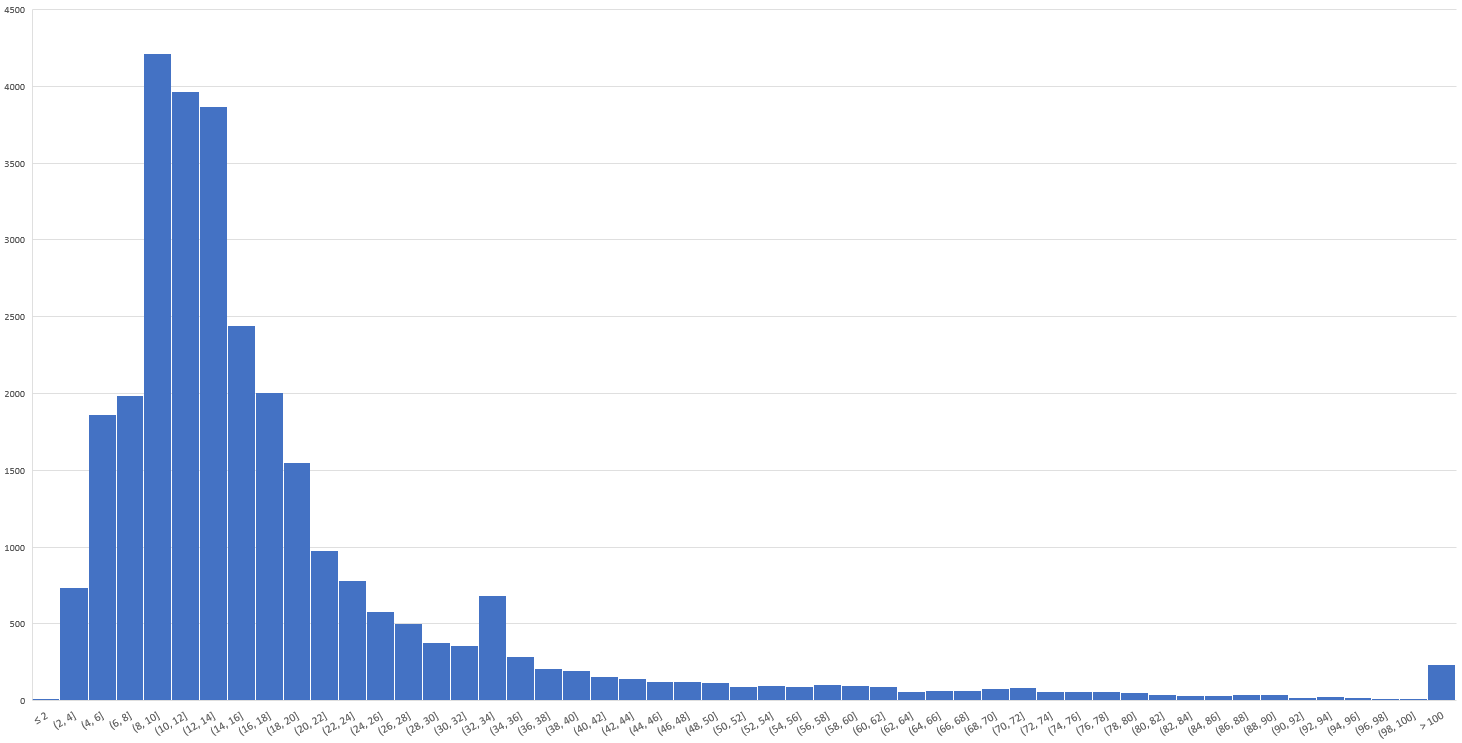
\includegraphics[width=\textwidth]{hist_ent_tot.png}
  \caption[Histograma de la longitud de totes les entitats]{Histograma de la longitud de totes les entitats. \\ (Creació pròpia)}
  \label{fig:histograma_entitats_total}
\end{figure}
